\documentclass[10pt]{article}

\input{/Users/gabesekeres/Dropbox/LaTeX_Docs/pset_preamble.tex}

\course{ECON 6200}
\pset{3}
\begin{document}
\maketitle

\begin{enumerate}
	\item Binary Variables IV estimator \begin{enumerate} \item Recall that the OLS estimator is defined by \[\hat{\beta} = \parl \frac{1}{n}\sum_{i=1}^n x_i^2\parr^{-1} \frac{1}{n}\sum_{i=1}^n x_iy_i\]which, in this case, since $x_i^2 = x_i$, simplifies to\[\hat{\beta} = \frac{\frac{1}{n}\sum_{i=1}^n x_iy_i}{\bar{x}} = \frac{\sum_{i=1}^n y_i \cdot \ones_{x_i = 1} + y_i \cdot 0 \cdot \ones_{x_i=0}}{\sum_{i=1}^n \ones_{x_i = 1}} = \frac{\sum_{i=1}^n y_i \cdot \ones_{x_i=1}}{\sum_{i=1}^n \ones_{x_i=1}} - \frac{\sum_{i=1}^n y_i \cdot \ones_{x_i=0}}{\sum_{i=1}^n \ones_{x_i=0}} = \bar{y}_1 - \bar{y}_0\]We also know that $\hat{\alpha} = \bar{y} - \hat{\beta}\bar{x}$, so\[\hat{\alpha} = \bar{y} - (\bar{y}_1-\bar{y}_0) \cdot \sum_{i=1}^n\ones_{x_i=x} = \bar{y} - \bar{y}_1\cdot \sum_{i=1}^n\ones_{x_i=x} = \bar{y}_0\]We additionally have that $\hat{y}_i = \hat{\alpha} + \hat{\beta} x_i$, so\begin{align*} \hat{y}_1 &= \bar{y}_0 + (\bar{y}_1 - \bar{y}_0)x_1 = \bar{y}_0 - \bar{y}_0 + \bar{y}_1 = \bar{y}_1 \\\hat{y}_0 &= \bar{y}_0 + (\bar{y}_1 - \bar{y}_0)x_0 = \bar{y}_0 \end{align*}where $x_1 = 1$ and $x_0 = 0$. \item $\hat{\beta}$ is not a credible estimate for the causal effect of $\beta$. If using a Malaria net is correlated with spending more on child health care, then there would be correlation between $x$ and $\varepsilon$. \item Since we have both truly random treatment and full compliance, there is now no way that $x$ and $\varepsilon$ are correlated. Thus, $\hat{\beta}$ does estimate the true causal effect of Malaria nets. \item We can use $z_i$ as an instrument for $x_i$, since validity and the exclusion restriction apply. Our estimator is now \[\hat{\beta} = (\expect ZX')^{-1}\expect ZY\]which becomes\[\hat{\beta}= \frac{\sum(y_i - \bar{y})(z_i - \bar{z})}{\sum(x_i-\bar{x})(z_i-\bar{z})} = \frac{\bar{y}_1 - \bar{y}_0}{\bar{x}_1 - \bar{x}_0}\]\end{enumerate}
	\item Measurement Error \begin{enumerate} \item We have that \[Y\opt + \eta = \beta_0 + \beta_1\cdot X\opt + \varepsilon \Longleftrightarrow Y\opt = \beta_0 + \beta_1\cdot X\opt + \varepsilon -\eta\]where we have that this estimator is valid since $\eta$ i.i.d. implies that $\expect(\varepsilon - \eta \mid X) = 0$, and we have spherical errors since $\expect ((\varepsilon - \eta)^2 \mid X) = \sigma_\varepsilon^2 + \sigma_\eta^2$. Asymptotically, our estimator has a similar distribution as the typical OLS estimator, which follows from central limit theorem: \[\sqrt{n}(\hat{\beta}-\beta) \todist \normal\parl 0 , \frac{\sigma_\varepsilon^2+\sigma_\eta^2}{\var(X\opt)}\parr\] \item OLS of $Y\opt$ on $X$ would yield the equation \[Y\opt = \beta_0 + \beta_1\cdot X\opt + \beta_1 \cdot \eta +\varepsilon\]where, since $\expect(\beta_1 \mid X\opt) \ne 0$, we no longer have that $\expect(\beta_1 \eta + \varepsilon \mid X\opt) = 0$. In this expression, we have that \[\hat{\beta}_1 = (X\opt X\opt)^{-1} X\opt  (\beta_1\cdot X\opt + \beta_1 \cdot \eta +\varepsilon)\]so \[\expect[\hat{\beta}_1] = \beta_1 + \underbrace{ (X\opt X\opt)^{-1}X\opt\varepsilon}_{=0} + \underbrace{ (X\opt X\opt)^{-1}X\opt \beta_1 \eta}_{\ne 0}\] so the bias of this estimator is the nonzero term, $ (X\opt X\opt)^{-1}X\opt \beta_1 \eta$. \item We now observe a second variable, $\bar{X} = X\opt + \nu$. We will use this variable as an instrument for $X$, which is valid since it is correlated with $X$ and uncorrelated with $\eta$. We have that \[\hat{\beta}_{IV} = (\bar{X}X)^{-1} \bar{X}(\beta_1 X +\beta_1\eta + \varepsilon) = \beta_1 + \underbrace{(\bar{X}X)^{-1}\beta_1\bar{X}\eta}_{=0} + \underbrace{(\bar{X}X)^{-1}\bar{X}\varepsilon}_{=0} = \beta_1\]So this estimator is unbiased. Further, since we have that defining $\rho_{X\bar{X}}$ as the covariance between $X$ and $\bar{X}$, the asymptotics of this estimator simplify to\[\sqrt{n}(\hat{\beta}_{IV} - \hat{\beta}) \todist \normal \parl 0 , \frac{\sigma_\varepsilon^2}{\rho_{X\bar{X}}^2 \sigma_X^2}\parr\] \end{enumerate}
	\item Empirical Exercise \\ \textbf{n.b.} I completed this exercise using Python since I don't have a Stata license and I'm morally opposed to using R. The code is \href{code}{below} \begin{enumerate} \item I recreated the columns in Hansen, which are: \begin{center} \begin{tabular}{c|c|c} Vars & 2SLS(b) & education \\\hline education & $0.1611$ &\\experience &$0.1193$ & $-0.4133$\\ experience$^2 / 100$ &$-0.2305$ & $0.0928$ \\ Black &$-0.1017$ &$-1.0063$\\ south &$-0.0950$ &$-0.2671$\\ urban &$0.1164$ & $0.3998$\\ public & & $0.4304$ \\ private & & $0.1226$ \\ p & $< 0.001$ & $< 0.001$ \\ F &$717.93$ & $525.80$ \end{tabular}\end{center} \item I added the variable, and the coefficient of interest (on \texttt{ed76}) changed from $0.1611$ to $0.1710$, a $6.15\%$ change. The full difference is below in the \href{output}{output section}. \item The results changed a lot when adding the additional instruments. The coefficient of interest moved to $0.0827$, a change of $48.66\%$. More importantly, the R-squared almost doubled, from $0.1430$ to $0.2876$. Graphically, we have Figure~\ref{fig} \begin{figure}[H]\centering 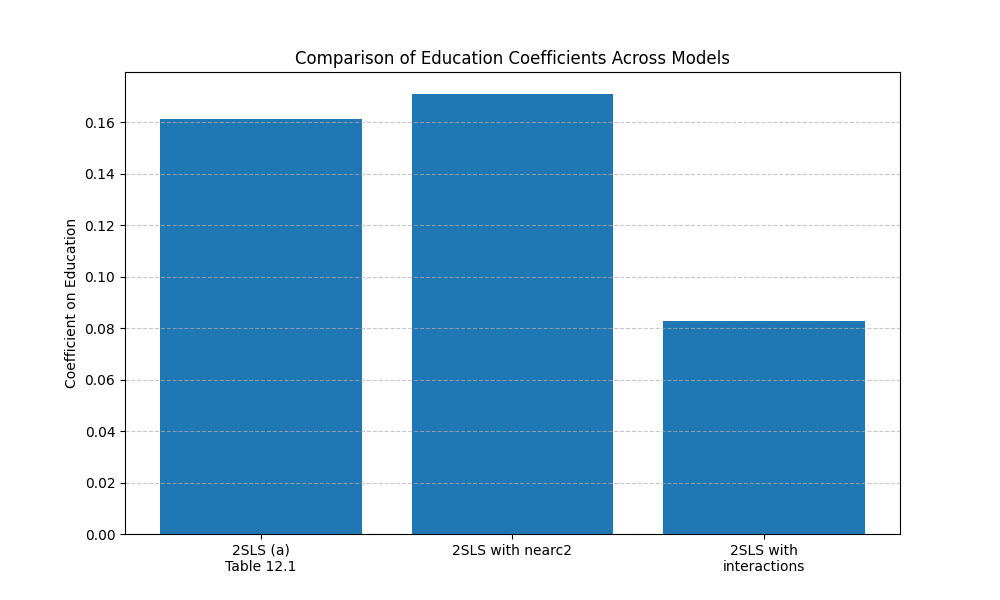
\includegraphics[width=10cm]{ps3_code/education_coefficients.png}\caption{Coefficient Comparison}\label{fig}\end{figure}\end{enumerate}
\end{enumerate}



\subsubsection*{Code}\label{code}

The code I used was:

\lstinputlisting[language=Python]{ps3_code/ps3_code.py}


\subsubsection*{Output}\label{output}

The raw output from the code was:
\begin{verbatim}
============== QUESTION 3.1 ==============

--- Table 12.1, Column 2SLS(a) ---
                          IV-2SLS Estimation Summary                          
==============================================================================
Dep. Variable:                lwage76   R-squared:                      0.1447
Estimator:                    IV-2SLS   Adj. R-squared:                 0.1430
No. Observations:                3010   F-statistic:                    717.93
Date:                Wed, Mar 05 2025   P-value (F-stat)                0.0000
Time:                        11:52:08   Distribution:                  chi2(6)
Cov. Estimator:                robust                                         
                                                                              
                             Parameter Estimates                              
==============================================================================
            Parameter  Std. Err.     T-stat    P-value    Lower CI    Upper CI
------------------------------------------------------------------------------
Intercept      3.2680     0.6821     4.7910     0.0000      1.9311      4.6049
exp76          0.1193     0.0182     6.5681     0.0000      0.0837      0.1549
exp76sq       -0.2305     0.0368    -6.2729     0.0000     -0.3026     -0.1585
black         -0.1017     0.0440    -2.3134     0.0207     -0.1879     -0.0155
south76       -0.0950     0.0217    -4.3717     0.0000     -0.1376     -0.0524
urban76        0.1164     0.0263     4.4327     0.0000      0.0650      0.1679
ed76           0.1611     0.0405     3.9804     0.0001      0.0818      0.2404
==============================================================================

Endogenous: ed76
Instruments: pub, priv
Robust Covariance (Heteroskedastic)
Debiased: False

--- Table 12.2, Final Column (Reduced Form for Education) ---
                            OLS Regression Results                            
==============================================================================
Dep. Variable:                   ed76   R-squared:                       0.476
Model:                            OLS   Adj. R-squared:                  0.475
Method:                 Least Squares   F-statistic:                     525.8
Date:                Wed, 05 Mar 2025   Prob (F-statistic):               0.00
Time:                        11:52:08   Log-Likelihood:                -6261.0
No. Observations:                3010   AIC:                         1.254e+04
Df Residuals:                    3002   BIC:                         1.259e+04
Df Model:                           7                                         
Covariance Type:                  HC1                                         
==============================================================================
                 coef    std err          z      P>|z|      [0.025      0.975]
------------------------------------------------------------------------------
const         16.6573      0.147    113.499      0.000      16.370      16.945
exp76         -0.4133      0.032    -12.904      0.000      -0.476      -0.350
exp76sq        0.0928      0.171      0.543      0.587      -0.242       0.428
black         -1.0063      0.088    -11.437      0.000      -1.179      -0.834
south76       -0.2671      0.079     -3.396      0.001      -0.421      -0.113
urban76        0.3998      0.085      4.717      0.000       0.234       0.566
pub            0.4304      0.086      4.994      0.000       0.261       0.599
priv           0.1226      0.101      1.210      0.226      -0.076       0.321
==============================================================================
Omnibus:                       12.456   Durbin-Watson:                   1.767
Prob(Omnibus):                  0.002   Jarque-Bera (JB):               12.583
Skew:                           0.158   Prob(JB):                      0.00185
Kurtosis:                       2.969   Cond. No.                         64.2
==============================================================================

Notes:
[1] Standard Errors are heteroscedasticity robust (HC1)

============== QUESTION 3.2 ==============

--- First Stage/Reduced Form with nearc2 added ---
                            OLS Regression Results                            
==============================================================================
Dep. Variable:                   ed76   R-squared:                       0.476
Model:                            OLS   Adj. R-squared:                  0.475
Method:                 Least Squares   F-statistic:                     460.2
Date:                Wed, 05 Mar 2025   Prob (F-statistic):               0.00
Time:                        11:52:08   Log-Likelihood:                -6260.6
No. Observations:                3010   AIC:                         1.254e+04
Df Residuals:                    3001   BIC:                         1.259e+04
Df Model:                           8                                         
Covariance Type:                  HC1                                         
==============================================================================
                 coef    std err          z      P>|z|      [0.025      0.975]
------------------------------------------------------------------------------
const         16.6343      0.150    111.215      0.000      16.341      16.927
exp76         -0.4128      0.032    -12.897      0.000      -0.476      -0.350
exp76sq        0.0895      0.171      0.524      0.600      -0.245       0.424
black         -1.0106      0.088    -11.490      0.000      -1.183      -0.838
south76       -0.2603      0.079     -3.299      0.001      -0.415      -0.106
urban76        0.3904      0.086      4.563      0.000       0.223       0.558
pub            0.4216      0.087      4.874      0.000       0.252       0.591
priv           0.1301      0.102      1.279      0.201      -0.069       0.329
nearc2         0.0677      0.074      0.911      0.362      -0.078       0.213
==============================================================================
Omnibus:                       12.199   Durbin-Watson:                   1.767
Prob(Omnibus):                  0.002   Jarque-Bera (JB):               12.319
Skew:                           0.156   Prob(JB):                      0.00211
Kurtosis:                       2.972   Cond. No.                         64.6
==============================================================================

Notes:
[1] Standard Errors are heteroscedasticity robust (HC1)

--- 2SLS with nearc2 added as an instrument ---
                          IV-2SLS Estimation Summary                          
==============================================================================
Dep. Variable:                lwage76   R-squared:                      0.1097
Estimator:                    IV-2SLS   Adj. R-squared:                 0.1079
No. Observations:                3010   F-statistic:                    691.41
Date:                Wed, Mar 05 2025   P-value (F-stat)                0.0000
Time:                        11:52:08   Distribution:                  chi2(6)
Cov. Estimator:                robust                                         
                                                                              
                             Parameter Estimates                              
==============================================================================
            Parameter  Std. Err.     T-stat    P-value    Lower CI    Upper CI
------------------------------------------------------------------------------
Intercept      3.1014     0.6883     4.5061     0.0000      1.7524      4.4503
exp76          0.1234     0.0184     6.7075     0.0000      0.0873      0.1594
exp76sq       -0.2313     0.0376    -6.1428     0.0000     -0.3051     -0.1575
black         -0.0917     0.0446    -2.0555     0.0398     -0.1792     -0.0043
south76       -0.0916     0.0220    -4.1581     0.0000     -0.1348     -0.0484
urban76        0.1113     0.0267     4.1722     0.0000      0.0590      0.1636
ed76           0.1710     0.0408     4.1877     0.0000      0.0910      0.2510
==============================================================================

Endogenous: ed76
Instruments: pub, priv, nearc2
Robust Covariance (Heteroskedastic)
Debiased: False

Comparison of coefficients with and without nearc2:
2SLS without nearc2 (ed76 coefficient): 0.1611
2SLS with nearc2 (ed76 coefficient): 0.1710
Difference: 0.0099
Percent change: 6.15%

============== QUESTION 3.3 ==============

--- 2SLS with additional instruments (interactions) ---
                          IV-2SLS Estimation Summary                          
==============================================================================
Dep. Variable:                lwage76   R-squared:                      0.2891
Estimator:                    IV-2SLS   Adj. R-squared:                 0.2876
No. Observations:                3010   F-statistic:                    1019.4
Date:                Wed, Mar 05 2025   P-value (F-stat)                0.0000
Time:                        11:52:08   Distribution:                  chi2(6)
Cov. Estimator:                robust                                         
                                                                              
                             Parameter Estimates                              
==============================================================================
            Parameter  Std. Err.     T-stat    P-value    Lower CI    Upper CI
------------------------------------------------------------------------------
Intercept      4.5873     0.1107     41.444     0.0000      4.3703      4.8042
exp76          0.0872     0.0071     12.361     0.0000      0.0733      0.1010
exp76sq       -0.2247     0.0320    -7.0277     0.0000     -0.2874     -0.1621
black         -0.1809     0.0180    -10.030     0.0000     -0.2162     -0.1455
south76       -0.1219     0.0154    -7.9085     0.0000     -0.1521     -0.0917
urban76        0.1569     0.0153     10.272     0.0000      0.1270      0.1869
ed76           0.0827     0.0062     13.295     0.0000      0.0705      0.0949
==============================================================================

Endogenous: ed76
Instruments: pub, priv, pubxage, pubxagesq, nearc2
Robust Covariance (Heteroskedastic)
Debiased: False

Comparison of coefficients with added interactions:
Original 2SLS (ed76 coefficient): 0.1611
2SLS with interactions (ed76 coefficient): 0.0827
Difference: -0.0784
Percent change: -48.66%
\end{verbatim}



\end{document}